% ! TeX program = xelatex
\documentclass[11.5pt]{beamer}
\usetheme{metropolis}

\usepackage{changepage}

\usepackage{xeCJK}
\setCJKmainfont{regular}[
    Path="fonts/simplified_chinese/noto_serif/",
    BoldFont=bold.otf
]
\xeCJKDeclareSubCJKBlock{Hangul}{"1100 -> "11FF, "3130 -> "318F, "A960 -> "A97F, "AC00 -> "D7AF, "D7B0 -> "D7FF}
\setCJKmainfont{regular}[
    Hangul,
    Path="fonts/korean/noto_serif/",
    BoldFont=bold.otf
]

\xeCJKDeclareSubCJKBlock{Kana}{"3040 -> "309F, "30A0 -> "30FF, "31F0 -> "31FF, "1B000 -> "1B0FF}
\setCJKmainfont{regular}[
    Kana,
    Path="fonts/japanese/noto_serif/",
    BoldFont=bold.otf
]



\title{\huge{Translate English Taiwan's Address To Chinese}}
\author{Hsiu-Hsuan(Jacky) Yeh}
\date{2024-03-17}
\begin{document}
\maketitle


\begin{frame}{Outline}
\tableofcontents
\end{frame}


\section{developing package, llm-research}
\begin{frame}{Functionalities}

\begin{enumerate}
    \item suppport few-shot learning, \cite{Brown2020}
    \item structured response in json format
    \item automatically resume from an unexpected interrupt
    \item MLflow integration
\end{enumerate}

\end{frame}


\begin{frame}{Prompt Template, System Message}
The purpose of the system message is to convey a specific context to the LLM,
guiding it to think or behave in a specific way. However, not all LLMs support
system messages. For example, to the best of my knowledge, Gemini, provided by
Google, does not support this functionalities.
\end{frame}


\begin{frame}{Prompt Template, System Message}
You are an experienced expert in translating English addresses to Traditional Chinese.
Your task is to translate the English address to Traditional Chinese using Json format. \newline

"Note: Do not include the country and postal code in your response." \newline
"Note: Use '臺' instead of '台' whenever possible; for example, '臺北市' is preferable to '台北市'." \newline
"Note: Translate '-' to '之'; for example, 'NO.42-3' should be translated as '42之3號', not '42-3號'." \newline
"Note: If the address is not in Taiwan, translate it as -1, refering to the 5th example."
\end{frame}


\begin{frame}[fragile]{Prompt Template, Human Message}
\begin{lstlisting}[language=Python]

human_template = """\
{instructions}
Translate the following address in Traditional Chinese:
{owner_address}
Output Instructions:
{output_instructions}
Besides, don't forget to escape a single quote in your response json string.\
"""
\end{lstlisting}

There are three keys in this message: instructions, owner\_address and
output\_instructions. instructions and output\_instructions are required by this
pacage to hold some necessary messages. owner\_address is the customizable
query key, but it should be one of the key of the input.
\end{frame}


\begin{frame}[fragile]{Setup The Prompt}
\begin{lstlisting}[language=Python]

from llm_research.model import Prompt

prompt = Prompt(LLMResponse, 'data/raw/prompt/system.json', 'data/raw/prompt/human.json')

\end{lstlisting}
\end{frame}


\begin{frame}[fragile]{Structured Output}
\begin{lstlisting}[language=Python]

from langchain_core.pydantic_v1 import BaseModel, Field

class LLMResponse(BaseModel):
    translated_address: str = Field(description="the translated address in Traditional Chinese")

\end{lstlisting}
\end{frame}


\begin{frame}[fragile]{Setup OpenAI LLM}
\begin{lstlisting}[language=Python]

from llm_research.model import OpenAILLM
model = OpenAILLM(model="gpt-4-1106-preview", temperature=0., timeout=120)

\end{lstlisting}

To check more parameters for controling ChatGPT, refer to the LangChain API
    documentation: \href{https://api.python.langchain.com/en/latest/chat_models/langchain_openai.chat_models.base.ChatOpenAI.html#langchain_openai.chat_models.base.ChatOpenAI}{ChatOpenAI}
\end{frame}


\begin{frame}{MLflow Integration}
\begin{figure}[H]
% \caption{Economy Category}
\centering
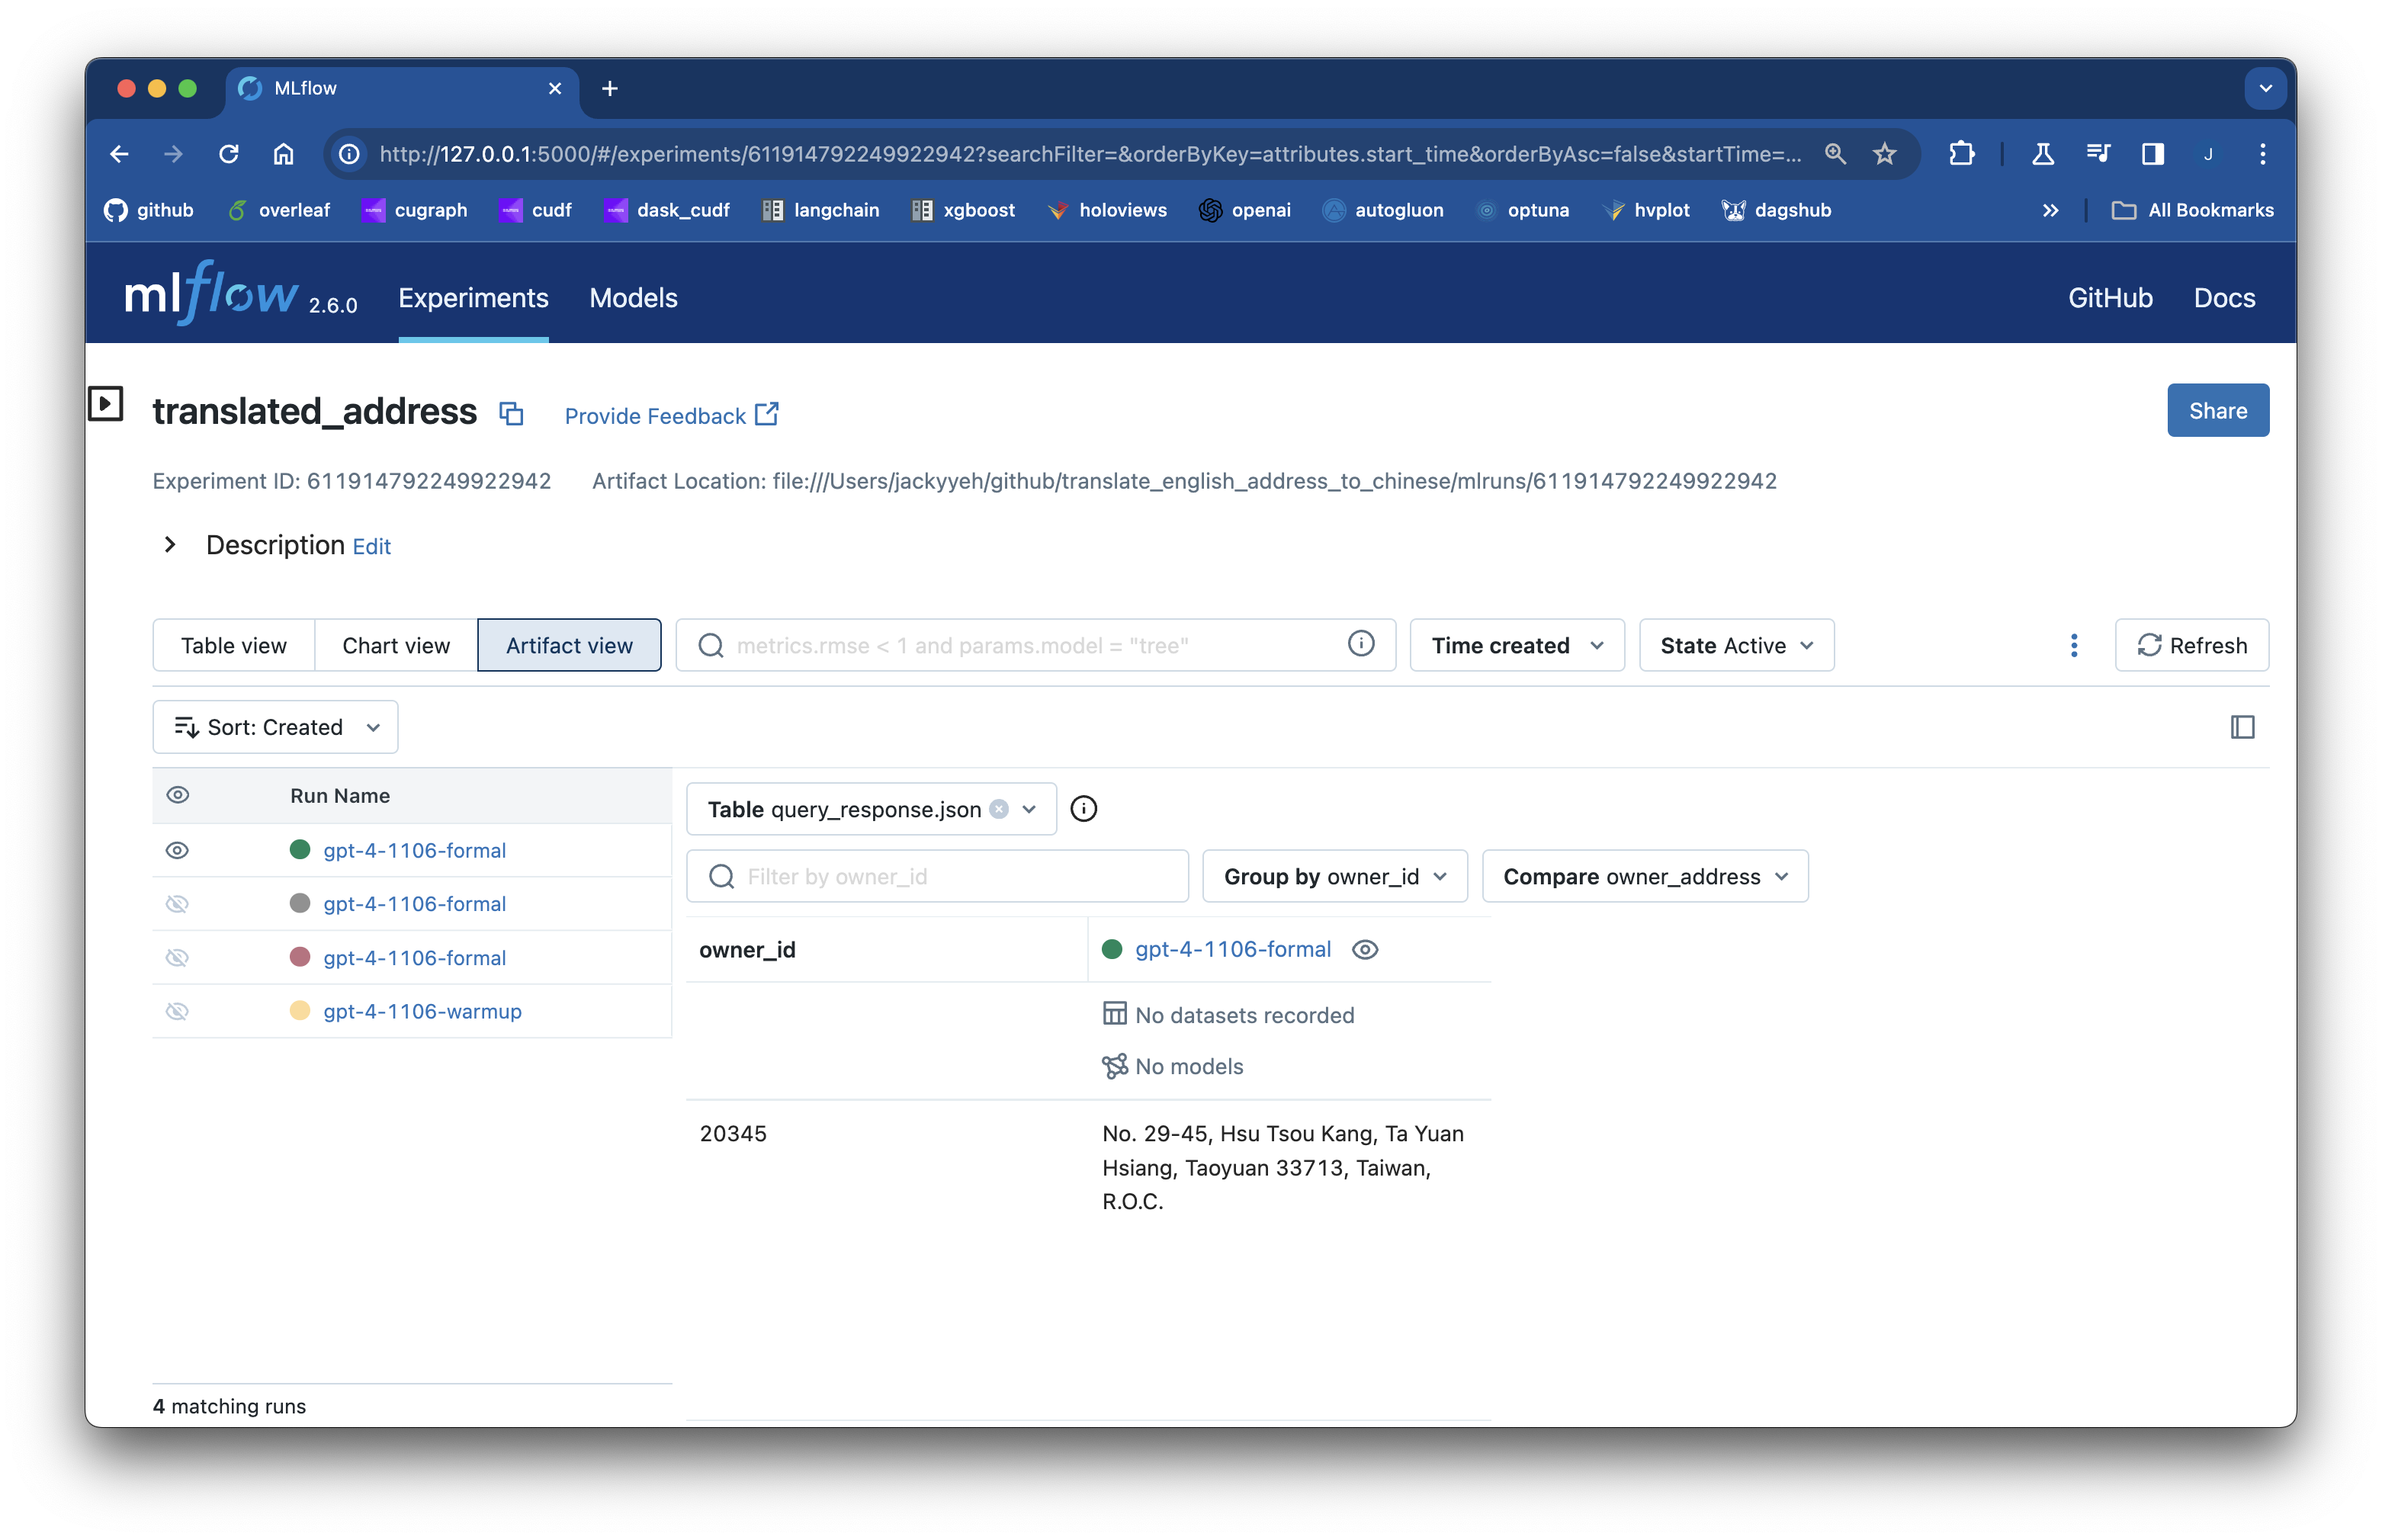
\includegraphics[width=11.5cm]{Figures/fig1.png}
\end{figure}
\end{frame}


\section{LangChain}
\begin{frame}{LangChain-Core}
The main component of LangChain-Core is LCEL, LangChain Expression Languages,
which involves several sub-components: prompt template, model, output parser,
etc.
\end{frame}

\begin{frame}{Ecosystem}
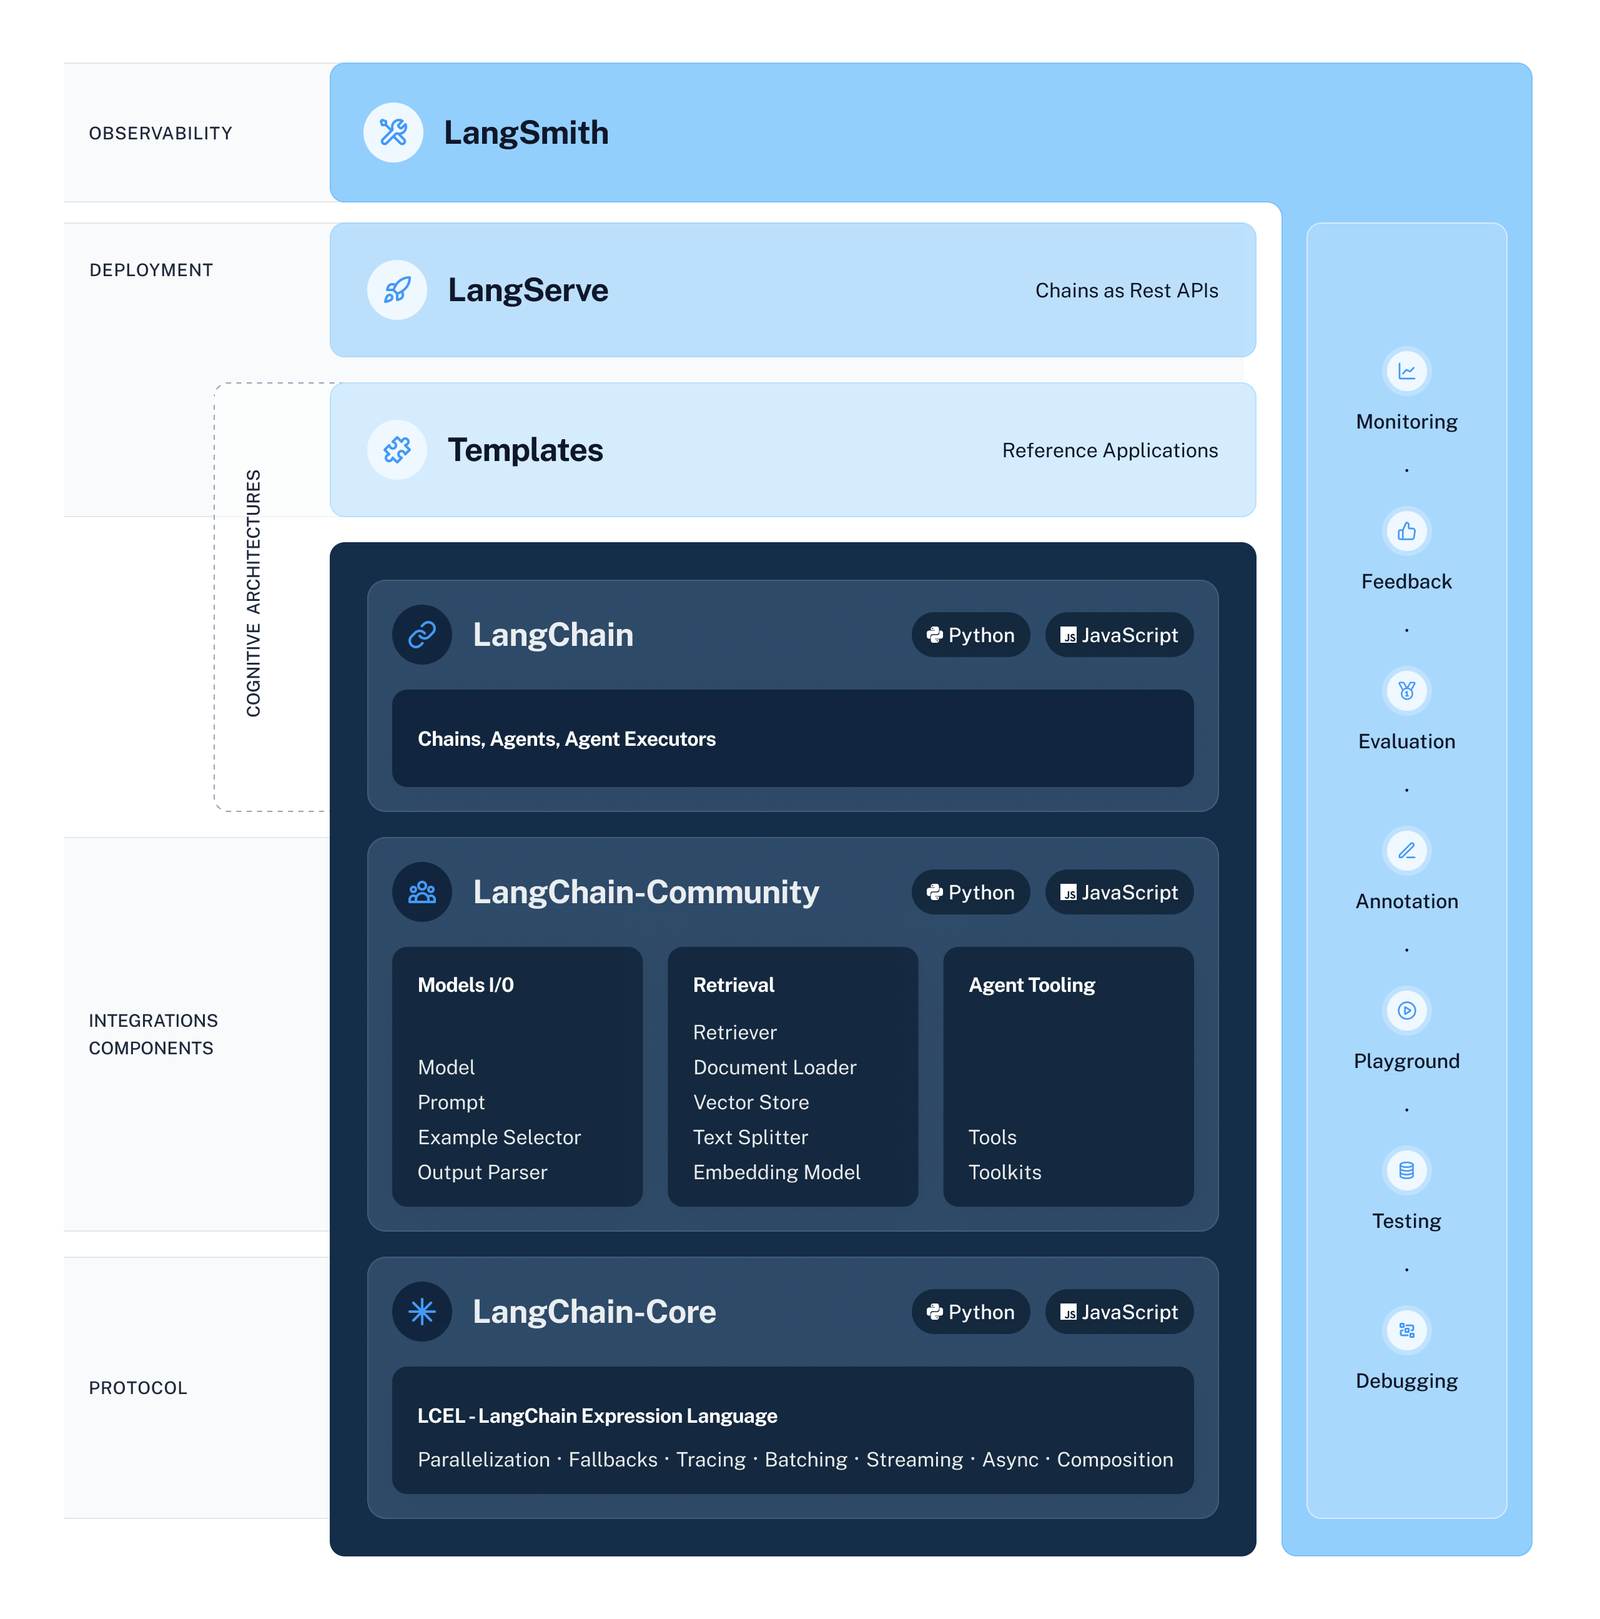
\includegraphics[width=11cm]{Figures/fig2.png}
\end{frame}

\begin{frame}{A Glimpse of LangChain-Core Documentation}
\begin{itemize}
    \item \href{https://python.langchain.com/docs/modules/model_io/prompts/quick_start}{Prompt Template}
    \item \href{https://python.langchain.com/docs/modules/model_io/prompts/few_shot_examples_chat}{Few-Shot Prompt}
    \item \href{https://python.langchain.com/docs/expression_language/why}{LCEL}
    \item \href{https://python.langchain.com/docs/integrations/chat/openai}{ChatOpenAI}
    \item \href{https://python.langchain.com/docs/modules/model_io/output_parsers/types/json}{Json Output Parser}
\end{itemize}
\end{frame}

\section{References}
\begin{frame}[allowframebreaks]{}
\renewcommand{\section}[2]{}%
\bibliography{/Users/jackyyeh/Library/texmf/bibtex/bib/Zotero.bib}
\end{frame}
\end{document}
